%!TEX program = xelatex

% Name              : mpilab_template.tex
% Author             : Jean-Pierre
% Version            : 0.1
% Created on       : 23.02.2016
% Last Edited on    : 1.03.2014
% License            : This file may be distributed and/or modified under the
%                              GNU Public License.
% Description      :  Sample template for MPI lab beamer

\documentclass{beamer}

\usetheme[mac]{course}
\usepackage{tikz}
\usetikzlibrary{mindmap,trees}
\title{MTE202 - Ordinary Differential Equations}
\subtitle{Mathematical Modelling  (Lecture 10)}
\author{Jean-Pierre Hickey}
\institute{Mechanical and Mechatronics Engineering}
\date{\today}
\usepackage{cancel}
\graphicspath{{./figs/}}
\begin{document}
{
\maketitle
}


\begin{frame}{Today's lecture}
\begin{itemize}
\item We take a step outside of MTE202.
\item Discuss mathematical modelling within a broader engineering context
\item Links together engineering/design, mathematics, and physics
\end{itemize}

\vspace{0.5cm}
Lecture plan:
\begin{itemize}
\item Contextualize mathematical modelling
\item Key Principles of mathematical modelling
\end{itemize}
\end{frame}





\begin{frame}{Mathematical Modelling}
\centering
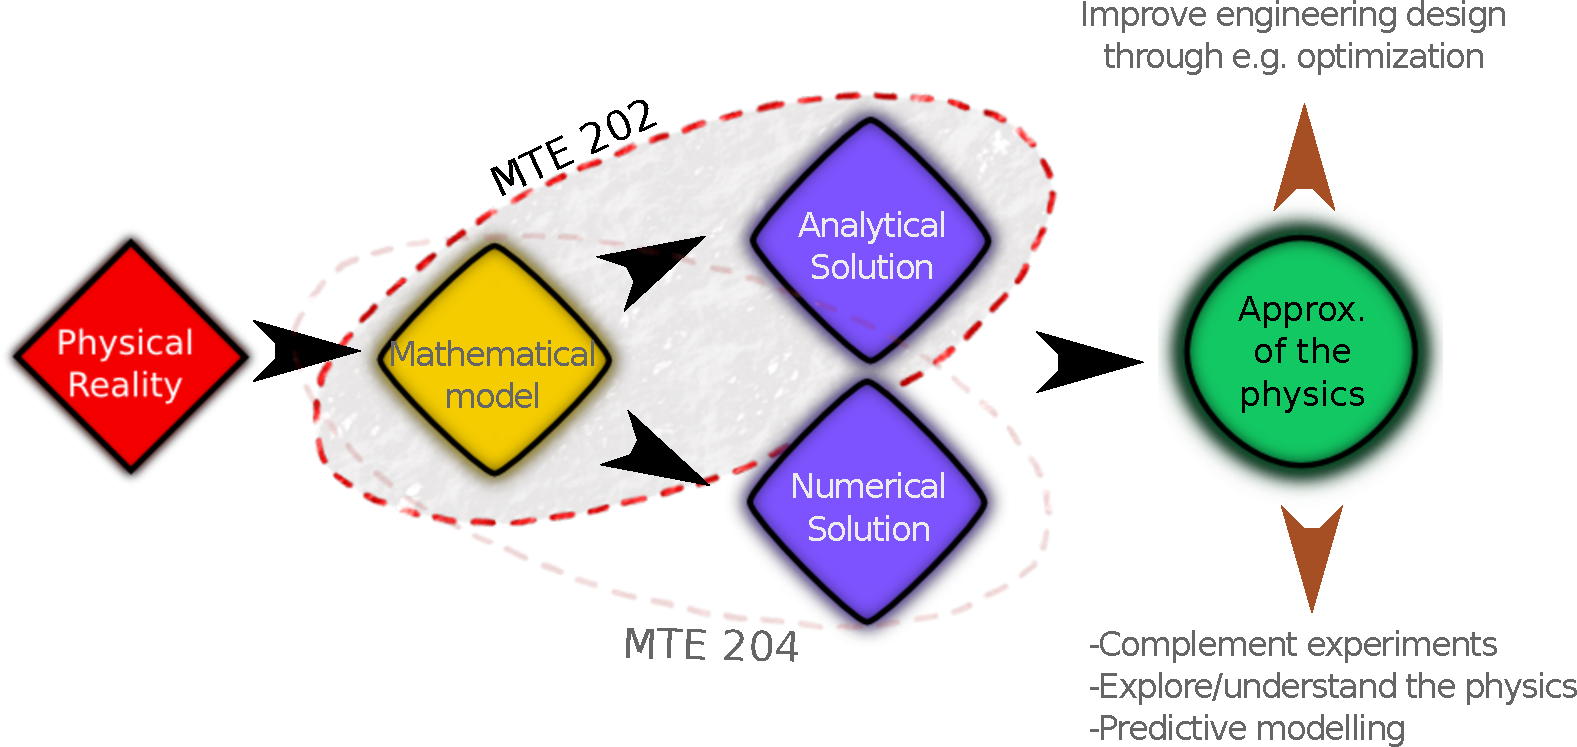
\includegraphics[width=0.6\textwidth]{../figs/ConceptMap.pdf} 
\begin{itemize}
\item The ability to develop mathematical models is (IMHO)  \textbf{one of the most important skills for an engineering undergrad}
\item The solution strategies to ODEs are tools, modelling is the assumption, \textbf{physical understanding is the objective}
\item Modelling is used to study heat transfer, fluid dynamics, material science etc. (..and banking and finance, quants?)
\end{itemize}
\end{frame}




\begin{frame}{Background}
\begin{itemize}
\item Generally, we need to create mathematical models from our physical understanding of a problem
\item The problem is rarely defined in mathematical terms
\item Often contains incomplete information, ambiguities, too much/too little information 
\item Need to use engineering intuition to focus on what is relevant and make judicious assumptions
\item Skills are transferable/generalizable (to other classes and/or other fields). The general approach towards mathematical modelling remains the same!
\item Problems seen in MTE202 will be academic/simple. The approach to a real problem is analogous.
\end{itemize}
\end{frame}



%\begin{frame}{Questions to answer}
%\begin{itemize}
%\item Why? What do we want to know?
%\item What is given?
%\item What are the governing physical principles?
%\item What are my assumptions?
%\item What will the model predict?
%\item How can I validate and verify the model?
%\end{itemize}
%
%\end{frame}



\begin{frame}{Key Principles of Mathematical Modelling}
\begin{itemize}
\item Dimensional Homogeneity and Consistency
\begin{itemize}
\item[-] The dimensions of a mathematical model must be consistent. If we model an equation for the mass balance of a system, all the terms must have dimensions of mass. Units must also be consistent.
\end{itemize}
\item  Abstraction and Scaling
\begin{itemize}
\item[-] The model should have the correct level of detail and abstraction for the desired output. 
\end{itemize}
\item  Conservation and Balance Principles
\begin{figure}
\centering
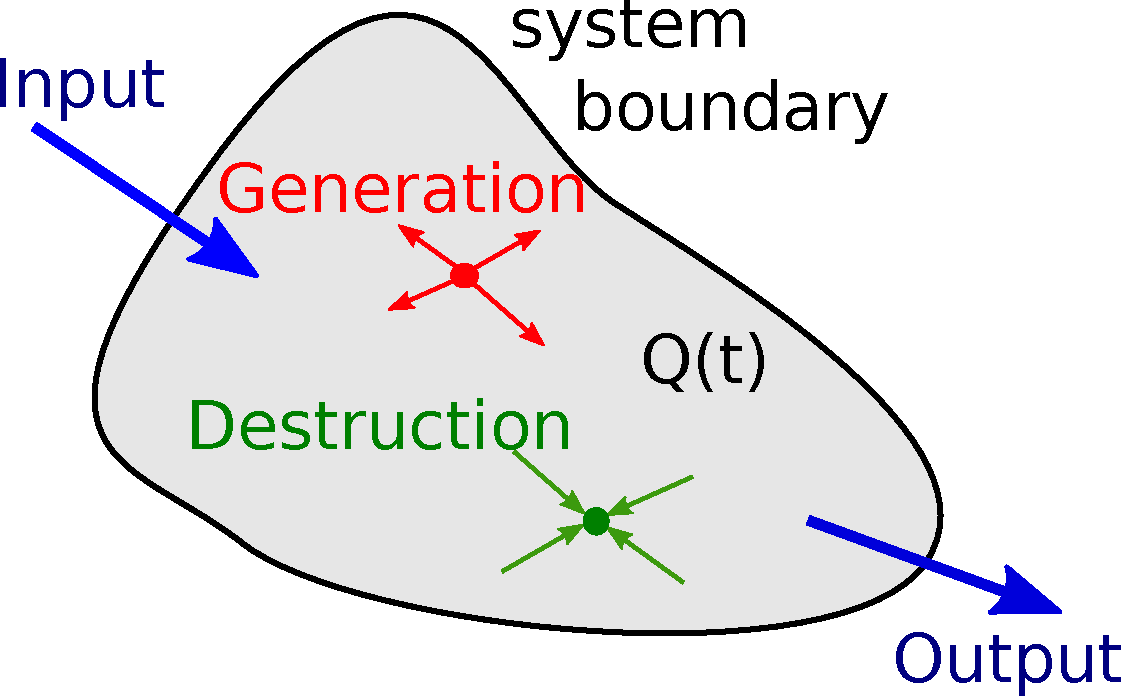
\includegraphics[width=0.4\textwidth]{figs/BC.pdf} 
\end{figure}
\end{itemize}
\end{frame}


%
%\begin{frame}{Liquid Rocket Engine Injector Head}
%Context:  A company wanted to know how well we can predict the heat load in a new injector design for liquid rocket engine combustion chamber.
%
%
%\begin{itemize}
%\item Why? What do we want to know?
%\item What is given?
%\item What are the governing physical principles?
%\item What are my assumptions?
%\item What will the model predict?
%\item How can I validate and verify the model?
%\end{itemize}
%
%\end{frame}
%

%
%
%
%\begin{frame}{Wood Pyrolysis}
%Pyrolysis is a thermochemical decomposition of organic material at elevated temperatures in the absence of oxygen.\\
%
%Video: https://youtu.be/7lfpLStXONo\\
%
%\begin{itemize}
%\item What do we want to know? 
%\begin{itemize}
%\item[-] How can we predict the physical behaviour of wood pyrolysis? Fire modellers would like to easily predict how wood pyrolyses.
%\end{itemize}
%
%\item What is given?
%\begin{itemize}
%\item[-] Typically, we know type of wood, moisture content of wood etc.
%\end{itemize}
%\item What are the governing physical principles?
%\begin{itemize}
%\item[-] This is where your job starts...
%\end{itemize}
%\end{itemize}
%
%\textbf{Exercise:}
%\begin{itemize}
%\item[-] Take about 10 minutes to analyze this problem in groups of 5-10
%\item[-] You may not have all the background needed (for heat transfer etc), but you are some of the smartest in the country!
%\item[-] The goal is not to get an exact answer but to develop the mindset needed for mathematical modelling
%\end{itemize}
%
%\end{frame}
%

\end{document}






